\documentclass[border=10pt]{standalone}
\usepackage{tikz}\usepackage{amsmath}\usetikzlibrary{arrows.meta}
\begin{document}
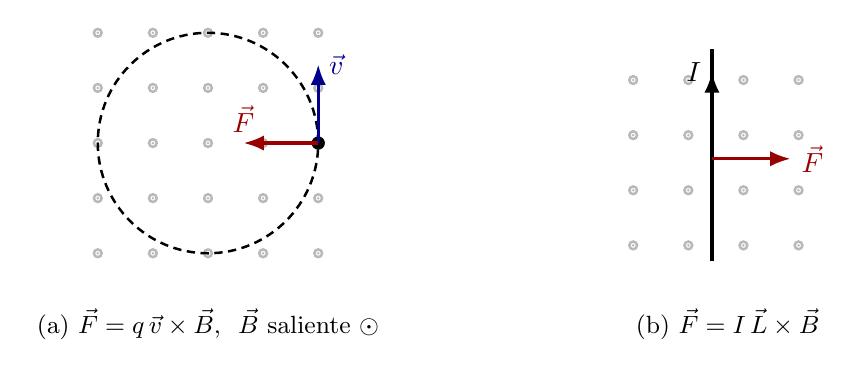
\begin{tikzpicture}[line width=0.9pt,>={Latex[length=2.6mm]}]
  % (a) carga en orbita circular, B saliente
  \foreach \x in {-1.4,-0.7,0,0.7,1.4} \foreach \y in {-1.4,-0.7,0,0.7,1.4}{
     \draw[gray!55] (\x,\y) circle(1.4pt); \fill[gray!55] (\x,\y) circle(0.5pt);}
  \draw[densely dashed] (0,0) circle(1.4);
  \fill (1.4,0) circle(2.4pt);
  \draw[->,blue!55!black,line width=1.2pt] (1.4,0)--(1.4,1.0) node[right]{$\vec v$};
  \draw[->,red!60!black,line width=1.2pt] (1.4,0)--(0.45,0) node[above]{$\vec F$};
  \node at (0,-2.3){\small (a) $\vec F=q\,\vec v\times\vec B$,\ \ $\vec B$ saliente $\odot$};
  % (b) fuerza sobre hilo con corriente
  \begin{scope}[xshift=6.4cm]
    \foreach \x in {-1.0,-0.3,0.4,1.1} \foreach \y in {-1.3,-0.6,0.1,0.8}{
       \draw[gray!55] (\x,\y) circle(1.4pt); \fill[gray!55] (\x,\y) circle(0.5pt);}
    \draw[line width=1.4pt] (0,-1.5)--(0,1.2);
    \draw[->,line width=1.2pt] (0,0.2)--(0,0.9) node[left]{$I$};
    \draw[->,red!60!black,line width=1.2pt] (0,-0.2)--(1.0,-0.2) node[right]{$\vec F$};
    \node at (0.2,-2.3){\small (b) $\vec F=I\,\vec L\times\vec B$};
  \end{scope}
\end{tikzpicture}
\end{document}
